\documentclass[a4paper,12pt]{report}
\usepackage[utf8]{inputenc}
\usepackage[sfdefault]{roboto}

\usepackage{titling}
\usepackage{graphicx}
\usepackage{wrapfig}
\usepackage{subcaption}
\usepackage{float}
\usepackage{fontawesome}
\usepackage{setspace}
\usepackage[export]{adjustbox}
\usepackage[margin=20mm]{geometry}
\usepackage{soul}

\usepackage{xcolor}
\definecolor{turbo_purple}{RGB}{112,105,160}
\definecolor{sponsor_bronze}{RGB}{205,127,50}
\definecolor{sponsor_silver}{RGB}{170,169,173}
\definecolor{sponsor_gold}{RGB}{212,175,55}

\usepackage{titlesec}
\titleformat{\section}[block]{\normalfont\huge\bfseries\centering}{}{1em}{}
\titleformat{\subsection}[display]{\normalfont\Large\bfseries\color{turbo_purple}}{}{1em}{}
\titleformat{\subsubsection}[display]{\normalfont\large\bfseries}{}{}{\vspace{-1.2em}}[\vspace{-0.9em}]

\usepackage{fancyhdr}
\pagestyle{fancy}
\usepackage{tikz}
\usetikzlibrary{calc}
\usepackage{tikzpagenodes}
\fancyfoot{}
\renewcommand{\headrulewidth}{0pt}
\setlength{\headheight}{25pt}
\rhead{\begin{tikzpicture}[remember picture,overlay]
\draw  let \p1=($(current page.north)-(current page header area.south)$),
      \n1={1.3 * veclen(\x1,\y1)} in
node [inner sep=0,outer sep=0,below left] 
      at (current page.north east){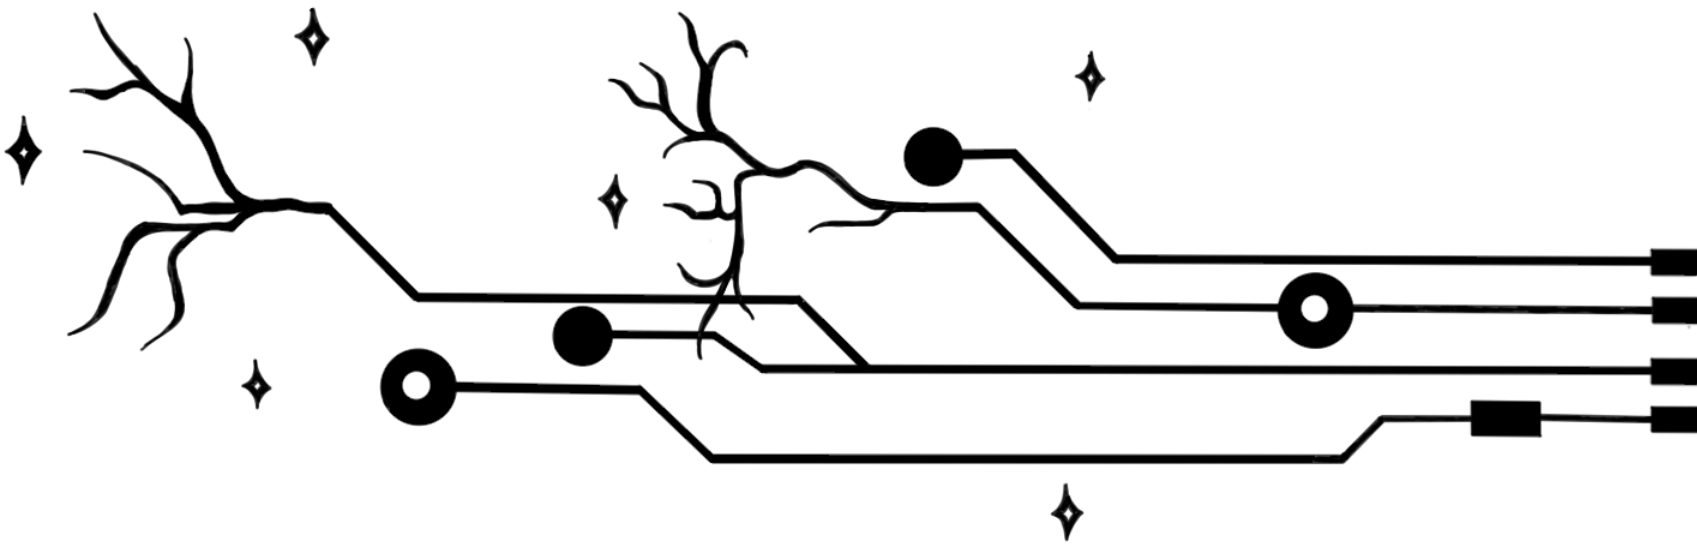
\includegraphics[height=\n1]{./photos/tech_dendrite_graphic_with_stars.png}};
\end{tikzpicture}}
\lfoot{\begin{tikzpicture}[remember picture,overlay]
\draw  let \p1=($(current page footer area.north)-(current page.south)$),
      \n1={1.5 * veclen(\x1,\y1)} in
node [inner sep=0,outer sep=0,above right] 
      at (current page.south west){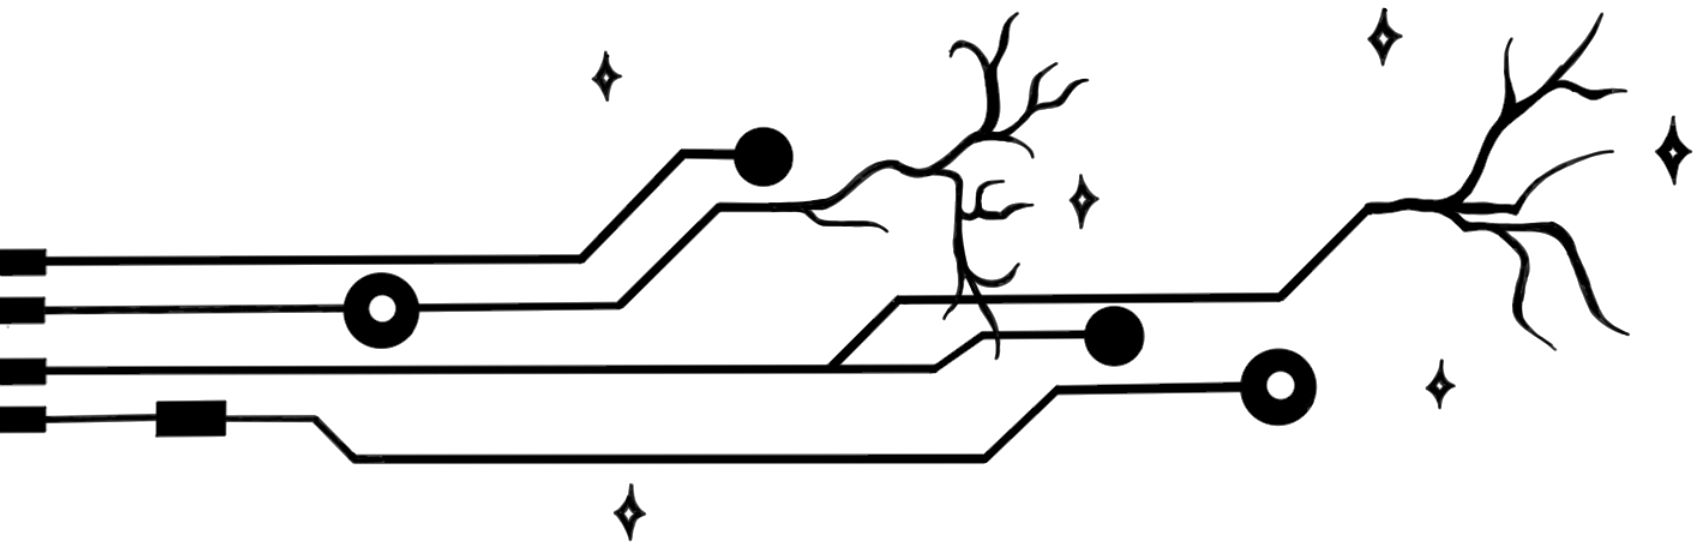
\includegraphics[height=\n1]{./photos/tech_dendrite_graphic_with_stars_flipped.png}};
\end{tikzpicture}}
\cfoot{\sffamily\selectfont\thepage}

\usepackage[hidelinks]{hyperref}
\hypersetup{colorlinks=false}

\begin{document}

\begin{titlepage}
    \newgeometry{right=0mm,left=0mm,top=20mm,bottom=0mm}
    \begin{center}
        \vspace*{15mm}
        
\includegraphics[width=0.8\paperwidth]{./photos/logo-fullform.png} \\
        \vspace{1cm}
        \Huge Sponsorship Prospectus \\
        \huge \textcolor{turbo_purple}{2024}

        \vspace*{30mm}
        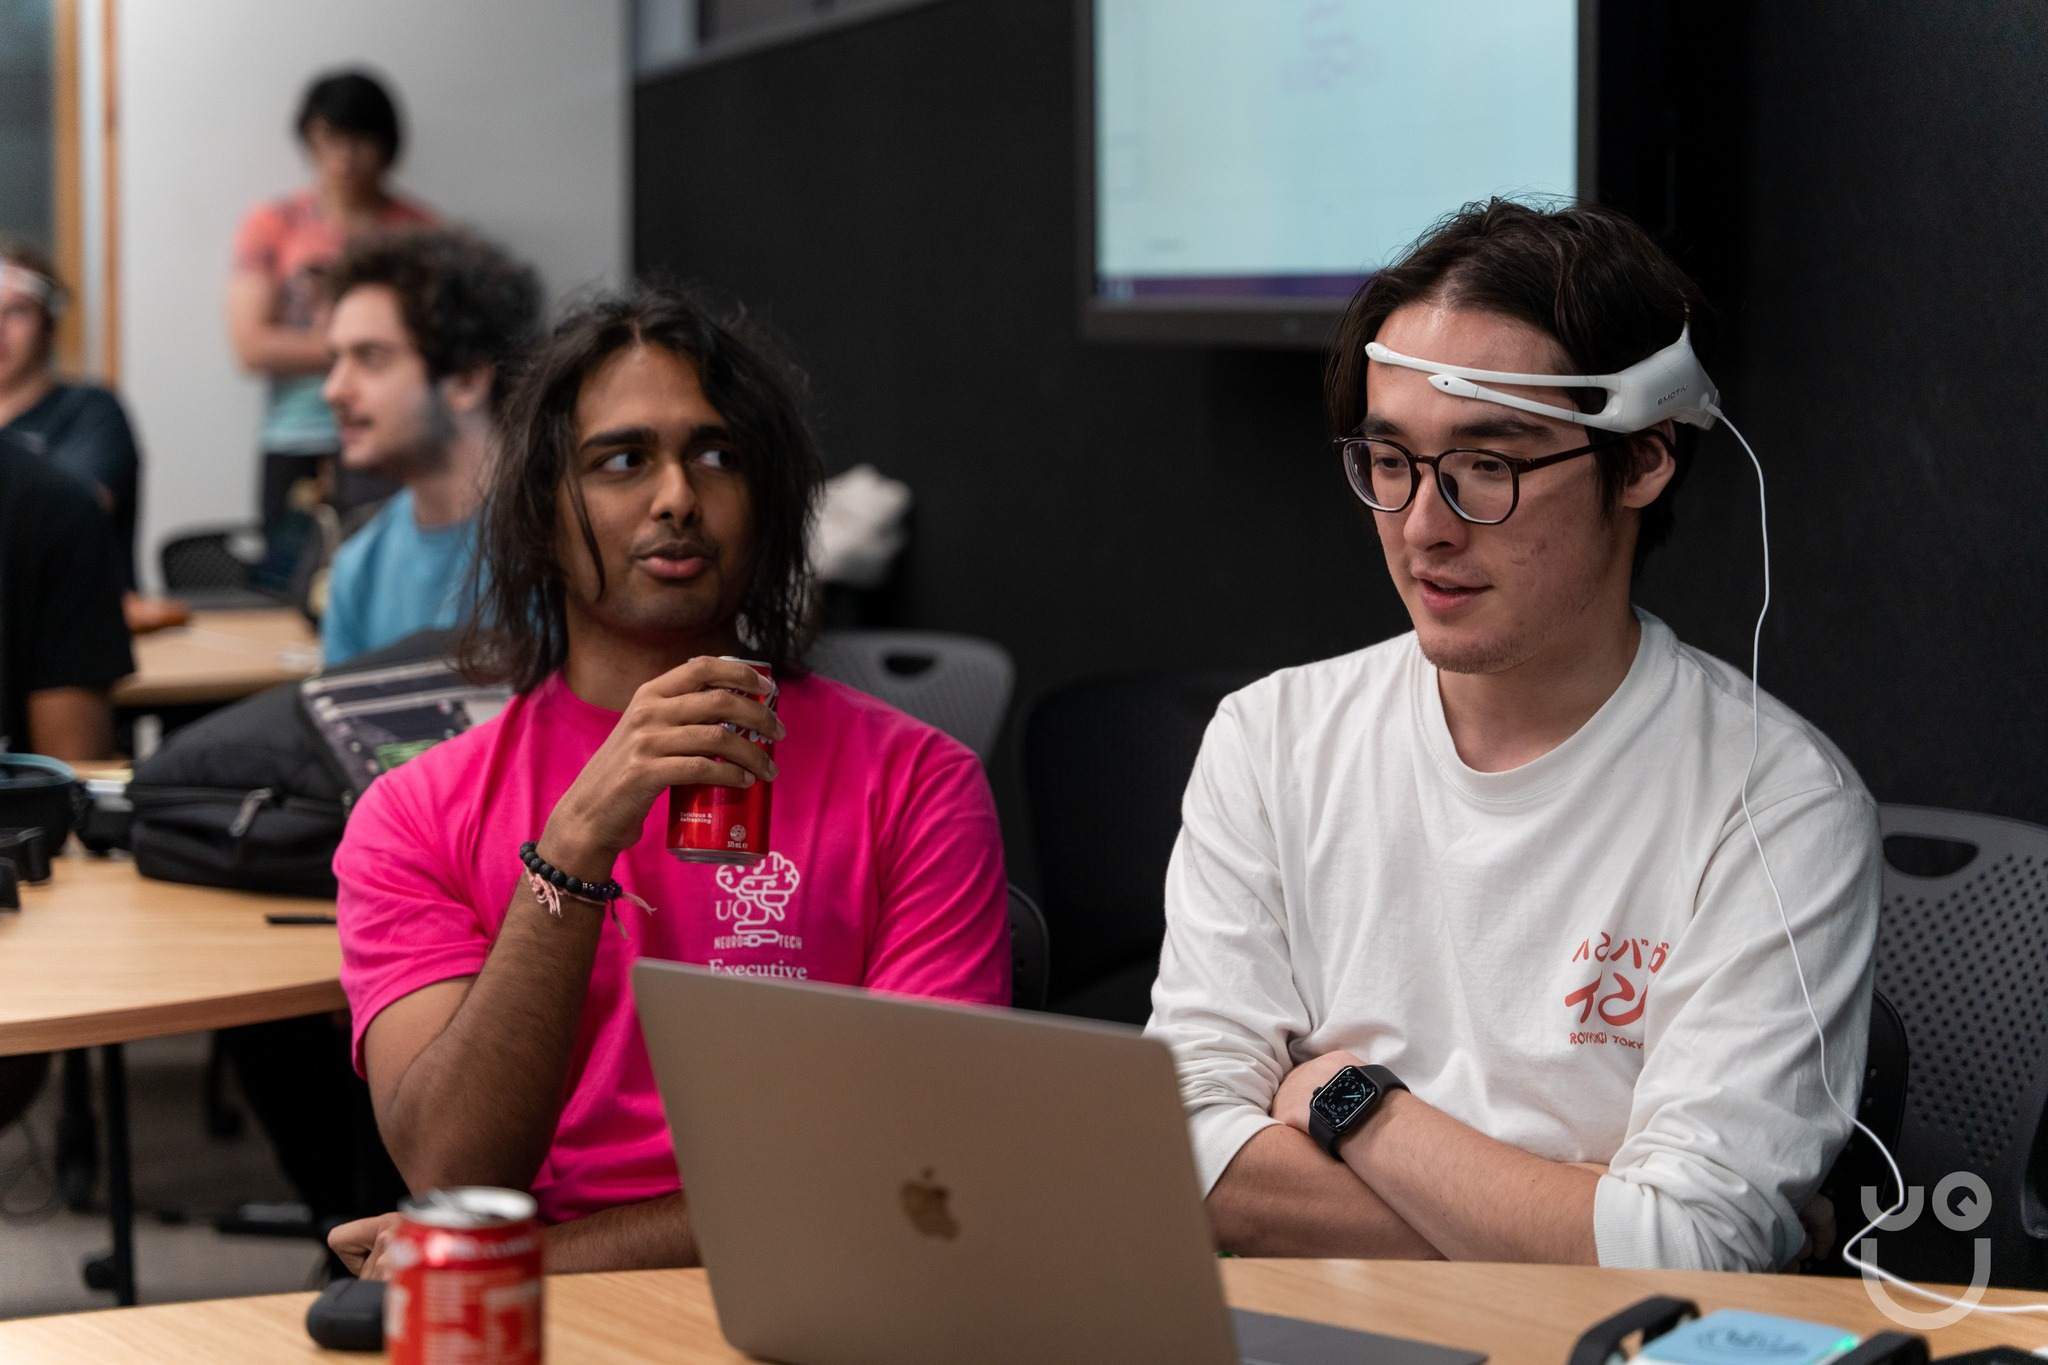
\includegraphics[height=0.32\paperheight]{./photos/emotiv-group-2p.jpg}
        \vfill

    \end{center}
    
\end{titlepage}
\restoregeometry

\section*{About UQ Neurotech}
% \subsection*{Our Philosophy}

\begin{wrapfigure}{r}{0.25\textwidth}
\vspace{-15pt}
% \raisebox{0pt}[\dimexpr\height-\baselineskip\relax]{
%     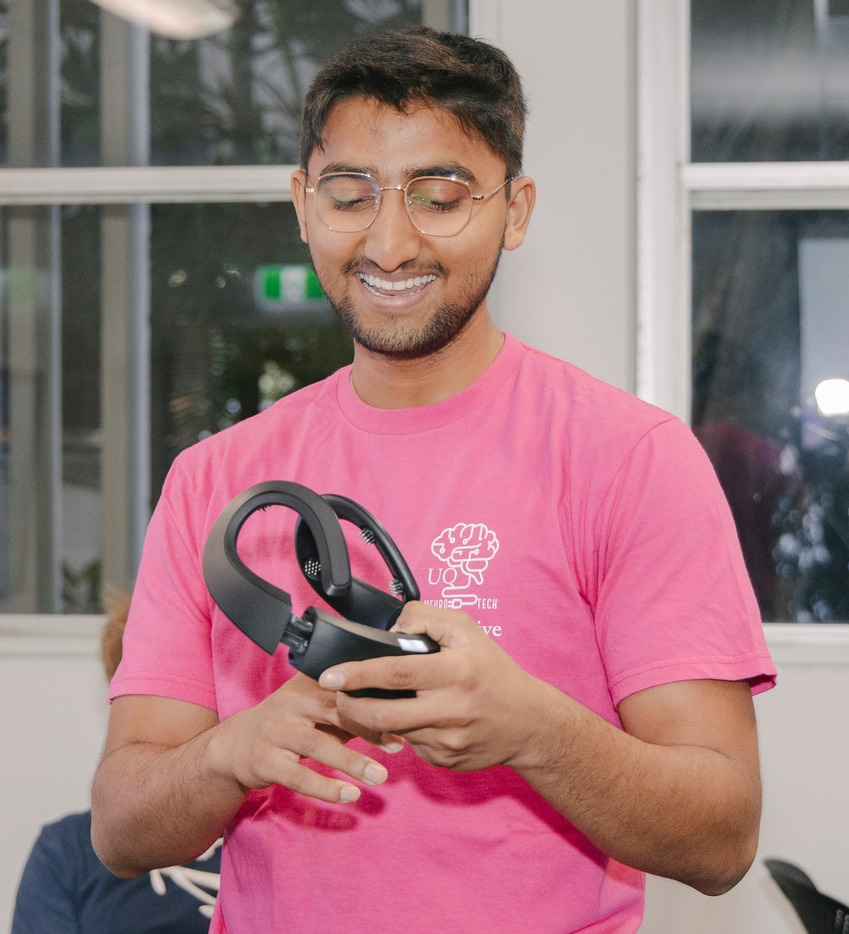
\includegraphics[width=0.95\linewidth]{./photos/jahan-with-crown-cropped.jpg}
% }
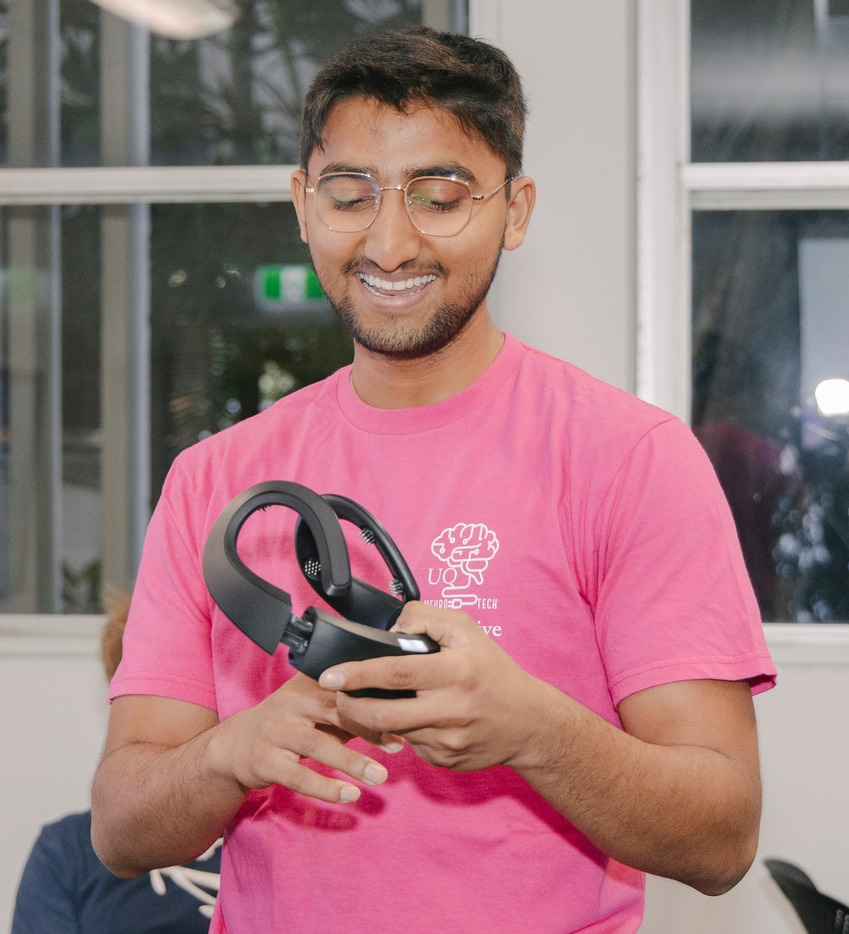
\includegraphics[width=0.95\linewidth]{./photos/jahan-with-crown-cropped.jpg}
\vspace{-10pt}
\end{wrapfigure}

We are the University of Queensland's Neuro-technology Club: A dynamic student-led
community for exploring the intersection between neuroscience, technology, ethics \& regulation,
AI \& deep learning, and related fields. 

We provide a platform for aspiring neuro-technologists to
connect at our workshops, seminars and team competitions. Our club is committed to
exploring the potential of neurotechnology, driving innovation, and shaping future
industry leaders.

\vspace{-1.5cm}

\subsection{Our Team}

Meet the UQ NeuroTech executive team — each member plays a vital role in driving the club’s mission, ensuring smooth operations, and fostering a thriving community.
\begin{itemize}
    \item \subsubsection{President}
    The President provides overall leadership for UQ NeuroTech, coordinating both internal operations and external relations. 
    They ensure the executive team functions cohesively, while remaining approachable and well-informed.

    \item \subsubsection{Secretary}
    The Secretary acts as the central point of communication across the club, managing internal coordination and 
    ensuring consistent messaging with members, executives, and external stakeholders.

    \item \subsubsection{Treasurer}
    The Treasurer manages the club’s financial affairs, maintaining accurate records and overseeing all financial 
    interactions with external partners.

    \item \subsubsection{Media Officer}
    The Media Officer leads promotional efforts and manages the club’s presence across social media 
    platforms to engage the community and promote events.

    \item \subsubsection{Development Team Leader}
    The Development Team Leader oversees the club's development initiatives, and organises our development team. 
    This includes scheduling dev meetings, introducing new team members, managing repositories and ensuring that all members of the team have 
    the resources they need to persue their projects.

    \item \subsubsection{Events Officer}
    The Events Officer organizes and coordinates general events, ensuring they are well-executed and align with the club’s goals and values.

    \item \subsubsection{General Executive}
    General Executives provide flexible support across different areas of the club, assisting wherever 
    needed to help ensure smooth operations. 
\end{itemize}


% \begin{figure}[H]
%     \centering
%     \begin{subfigure}{0.32\linewidth}
%         \includegraphics[width=0.99\linewidth]{./Photos/Welcome-20.jpg}
%     \end{subfigure}
%     \begin{subfigure}{0.28\linewidth}
%         \includegraphics[width=0.99\linewidth]{./Photos/2023Sem2EAITExpo1.jpg}
%     \end{subfigure}
%     \begin{subfigure}{0.32\linewidth}
%         \includegraphics[width=0.99\linewidth]{./Photos/Welcome-14.jpg}
%     \end{subfigure}
% \end{figure}

\newpage

\section*{Our History}

(intro paragraph - oververview of the year, what we did, how many members we had, etc.)

\vspace{-1cm}

\subsection{Welcome Evening}
To mark the beginning of our affiliation as a club, we organized a social event and
club introduction. The evening featured a presentation outlining UQ Neurotech's
plans for the semester and exciting updates in Neurotechnology. Following the
presentation, we fostered a sense of community with a pizza night, encouraging
conversations and bonding among members.

\begin{figure}[H]
    \centering
    \begin{subfigure}{0.32\linewidth}
        
\includegraphics[width=0.99\linewidth]{./photos/placeholder.JPG}
    \end{subfigure}
    \begin{subfigure}{0.32\linewidth}
        
\includegraphics[width=0.99\linewidth]{./photos/placeholder.jpg}
    \end{subfigure}
    \begin{subfigure}{0.32\linewidth}
        
\includegraphics[width=0.99\linewidth]{./photos/placeholder.JPG}
    \end{subfigure}
\end{figure}

\vspace{-2cm}

\subsection{Neurotech Showcase Night}
UQ Neurotech hosted a demonstration day to exhibit the cutting-edge technology at
our disposal. The showcased devices included Neurosity Cown EEG, Emotive Insight,
and Emotiv Epoch. Looking ahead, we aspire to feature even more advanced
technology and ongoing research projects at future events.

\vspace{-1.8cm}

\subsection{Biomedical Industry and Research Showcase}
In collaboration with seven other societies, UQ Neurotech orchestrated a Biomedical
Industry Networking Night. This event brought together over 20 companies,
researchers, and a diverse audience of 70+ students. The showcase was a resounding
success, shedding light on the myriad opportunities in BioTech in Queensland and
beyond.

\begin{figure}[H]
    \centering
    \begin{subfigure}{0.32\linewidth}
        
\includegraphics[width=0.99\linewidth]{./photos/placeholder.jpg}
    \end{subfigure}
    \begin{subfigure}{0.32\linewidth}
        
\includegraphics[width=0.99\linewidth]{./photos/placeholder.jpg}
    \end{subfigure}
    \begin{subfigure}{0.32\linewidth}
        
\includegraphics[width=0.99\linewidth]{./photos/placeholder.jpg}
    \end{subfigure}
\end{figure}

\vspace{-1.8cm}

\subsection{Mind-Bot Race 2023}
(paragraph)

\begin{figure}[H]
    \centering
    \begin{subfigure}{0.42\linewidth}
        
\includegraphics[width=0.99\linewidth]{./photos/placeholder.jpg}
    \end{subfigure}
    \begin{subfigure}{0.42\linewidth}
        
\includegraphics[width=0.99\linewidth]{./photos/placeholder.jpg}
    \end{subfigure}
\end{figure}
\newpage

\subsection{EVENT NAME} 
(paragraph)
\begin{figure}[H]
    \centering
    \begin{subfigure}{0.32\linewidth}
        
\includegraphics[width=0.99\linewidth]{./photos/placeholder.jpg}
    \end{subfigure}
    \begin{subfigure}{0.32\linewidth}
        
\includegraphics[width=0.99\linewidth]{./photos/placeholder.jpg}
    \end{subfigure}
    \begin{subfigure}{0.32\linewidth}
        
\includegraphics[width=0.99\linewidth]{./photos/placeholder.jpg}
    \end{subfigure}
\end{figure}

\begin{figure}[H]
    \centering
    \begin{subfigure}{0.32\linewidth}
        
\includegraphics[width=0.99\linewidth]{./photos/placeholder.jpg}
    \end{subfigure}
    \begin{subfigure}{0.32\linewidth}
        
\includegraphics[width=0.99\linewidth]{./photos/placeholder.jpg}
    \end{subfigure}
\end{figure}

\subsection*{School Outreach}
(paragraph)

%% End Update Section ------------------------------------------------------------------------------------
\newpage

\section*{UQ Neurotech in 2026}
\subsection*{Goals}
text
% End Section ------------------------------------------------------------------------------------
% Add New photos ------------------------------------------------------------------------------------
\begin{figure}[H]
    \centering
    \begin{subfigure}{0.32\linewidth}
        
\includegraphics[width=0.99\linewidth]{./photos/placeholder.jpg}
    \end{subfigure}
    \begin{subfigure}{0.32\linewidth}
        
\includegraphics[width=0.99\linewidth]{./photos/placeholder.jpg}
    \end{subfigure}
    \begin{subfigure}{0.32\linewidth}
        
\includegraphics[width=0.99\linewidth]{./photos/placeholder.jpg}
    \end{subfigure}
\end{figure}

\subsection*{Mind-Bot Race}
(paragraph)

\subsection*{Competitions}
(paragraph)

\subsection*{Hackathon}
(paragraph)

\subsection*{Development Team \& Workshops}
(paragraph)

\subsection*{Regular Talks and Seminars} 
(paragraph)

\newpage

\subsection*{Workshops}

Proposed workshops:

\begin{itemize}
    \item blah
    \item blah blah
\end{itemize}

\begin{figure}[H]
    \centering
    
\includegraphics[width=0.42\linewidth]{./photos/placeholder.jpg}
    
\includegraphics[width=0.42\linewidth]{./photos/placeholder.jpg}
    
\includegraphics[width=0.42\linewidth]{./photos/placeholder.jpg}
    
\includegraphics[width=0.42\linewidth]{./photos/placeholder.jpg}
\end{figure}


\newpage

% ----- REPLACE IMAGE -----------------%
\begin{figure}[H]
    \centering
    
\includegraphics[width=0.9\linewidth]{./photos/placeholder.jpg}
\end{figure}

\subsection*{School Outreach}
(paragraph)

\subsection*{Inter-Society and Inter-University Events}
We understand that tertiary study is about far more than just your classes, it's also the connections and friendships you make while undertaking study.
Next year, we are committed to building even stronger relationships with other student societies both at the University of Queensland and beyond.

\newpage

\subsection*{Neurotechnology Newsletter}

\begin{itemize}
    \item Also maybe meantion UQ Neurotech alumni study advice
    \item Meantion these will be resources for the UQ community to access on our website
    \item Also meantion somewhere in this prospectus our dedication to open source and sharing 
    our resources with the wider community via our github page
\end{itemize}

\subsection*{External Competitions}
(paragraph)


\begin{figure}[H]
    \centering
    
\includegraphics[width=0.65\linewidth]{./photos/placeholder.jpg}
\end{figure}

\newpage

\section*{Partnering with UQ NeuroTech}
\large
We offer a number of sponsorship packages which are laid out below. The prices provided are annual figures, quoted in AUD.
\normalsize

\subsection*{
    
\includegraphics[width=1em]{./photos/logo.png}
    \textcolor{sponsor_bronze}{Bronze Tier (\$250)}
}
text
\subsection*{
    
\includegraphics[width=1em]{./photos/logo.png}
    \textcolor{sponsor_silver}{Silver Tier (\$1,000)}
}
text


\subsection*{
    
\includegraphics[width=1em]{./photos/logo.png}
    \textcolor{sponsor_gold}{Gold Tier (\$4,000)}
}
text

\subsection*{
    
\includegraphics[width=1em]{./photos/logo.png}
    \textcolor{turbo_purple}{Purple Tier (\$10,000)}
}
text


\subsection{\textit{*Disclaimer}}
text
\newpage

\section*{Contact Us}
\begin{figure}[H]
    \centering
    
\includegraphics[width=0.9\linewidth]{./photos/placeholder.jpg}
\end{figure}

\large
\onehalfspacing
You can contact us through any of the following platforms: \\
\faLink{} \href{https://uqneurotech.com}{uqneurotech.com} \\
\faEnvelope{} \href{mailto:contact@uqneurotech.com}{contact@uqneurotech.com} \\
\faFacebookSquare{} \href{https://www.facebook.com/uqneurotech}{UQ NeuroTech} \\
\faLinkedinSquare{} \href{https://www.linkedin.com/company/uq-neurotech/}{UQ NeuroTech} \\
\faGithubSquare{} \href{https://github.com/UQNeuroTech}{UQNeuroTech} \\
\faYoutubePlay{} \href{https://www.youtube.com/@UQNeuroTech}{UQ NeuroTech} \\
\faInstagram{} \href{https://www.instagram.com/uqneurotech/}{uqneurotech} \\
We look forward to hearing from you!

\end{document}
